%% MOCASSIN_octree_vs_patch.tex
%% Build:  pdflatex MOCASSIN_octree_vs_patch.tex
%% (compile from this directory so my_memo.cls is found)

\documentclass[11pt,a4paper]{my_memo}

\usepackage{listings}
\usepackage{booktabs}
\usepackage{tikz}
\usetikzlibrary{positioning,shapes,arrows.meta,fit,backgrounds}
\usepackage{xcolor}

\lstset{
  basicstyle=\ttfamily\footnotesize,
  keywordstyle=\bfseries\color{blue!60!black},
  commentstyle=\color{gray!80!black}\itshape,
  stringstyle=\color{red!60!black},
  showstringspaces=false,
  breaklines=true,
  language=Fortran,
  columns=fullflexible,
  frame=single,
  framesep=4pt,
  rulecolor=\color{gray!40},
  xleftmargin=8pt,
  xrightmargin=4pt,
  belowskip=4pt,
  aboveskip=4pt,
}

\title{MOCASSIN Spatial Refinement: Patch-Based AMR vs.\ Octree}
\author{K.\ Seon}
\date{2026 May 1}

\begin{document}
\maketitle

\section{Motivation}

MOCASSIN is a Monte Carlo photo-ionisation and dust radiative-transfer code
built on a Cartesian grid with optional nested refinement.  The current
refinement strategy --- a flat list of independent rectangular sub-grids
linked by parent pointers --- has served well for the historical use cases
(planetary nebulae, isolated H\,\textsc{ii} regions) but is ill suited to
problems demanding adaptive resolution: deeply nested ionisation fronts,
multi-scale dust geometries, or shock-driven structures whose location is
unknown a priori.  An octree replacement is therefore under consideration.

The purpose of this memo is to lay out the existing data structures and
algorithms in enough detail that the necessary changes for an octree
transition are visible at a glance, and to document where the equivalence
between the two designs breaks down.

\section{Current Structure: Patch-Based Nested Rectilinear AMR}

\subsection{Grid container}

The active grid is held in a flat Fortran array,
\begin{lstlisting}
type(grid_type) :: grid3D(maxGrids)   ! mocassin.f90
integer         :: nGrids             ! number of grids in use
\end{lstlisting}
\begin{sloppypar}
Each \texttt{grid\_type} (defined in \texttt{common\_mod.f90:267--350}) is a
fully self-contained Cartesian grid: it owns its own resolution
$(n_x, n_y, n_z)$, face-aware coordinate arrays
\texttt{xFace}, \texttt{yFace}, \texttt{zFace}, an active-cell indicator
$\mathcal{A}(i,j,k)$, and the entire suite of cell-by-cell physical state arrays
(\texttt{Hden}, \texttt{Ne}, \texttt{Te}, \texttt{ionDen}, \texttt{Jste},
\texttt{Jdif}, \texttt{opacity}, \texttt{escapedPackets}, $\ldots$),
which are stored as one-dimensional arrays of length \texttt{nCells} indexed
by the active map.
\end{sloppypar}

The hierarchy is encoded by a single integer per grid,
\texttt{motherP}, which points to the index of the parent grid in
\texttt{grid3D}.  The root grid has \texttt{motherP\,=\,1}; sub-grids carry
\texttt{motherP\,>\,1}.  The mother grid records the cell range
$[i_0,i_1]\times[j_0,j_1]\times[k_0,k_1]$ that each child covers in
\texttt{motherX}, \texttt{motherY}, \texttt{motherZ}.

\subsection{Active map and child dispatch}

The integer 3D array $\mathcal{A}(i,j,k)$ encodes three states in a single
field:
\begin{equation}
   \mathcal{A}(i,j,k) =
   \begin{cases}
      n > 0 & \text{cell is active; } n \text{ is the flat index into cell-by-cell arrays,} \\
      0     & \text{cell is inactive (outside density cut),} \\
      -g    & \text{cell is covered by sub-grid } g.
   \end{cases}
\end{equation}
Mother-grid cells overlapped by a sub-grid are marked with the negation of
the child's grid index, so that traversal logic can dispatch with a single
sign test.

\subsection{Refinement specification}

Refinement is \emph{static} and \emph{user-defined} at run time.  The input
file declares
\begin{lstlisting}
multiGrids 2 'input/subgrid.in'
\end{lstlisting}
and \texttt{subgrid.in} contains, per child, a fixed-extent rectilinear
patch:
\begin{lstlisting}
<gridID> <nx> <ny> <nz> '<density.dat>' <fillingFactor>
<xmin> <xmax> <ymin> <ymax> <zmin> <zmax>
\end{lstlisting}
The user is responsible for choosing both the location and the resolution
of each sub-grid; the code does not adapt at run time.

\subsection{Photon traversal}

Cell-to-cell ray marching uses Amanatides--Woo three-dimensional digital
differential analysis (3D-DDA) on the face-aware coordinate arrays
(\texttt{dda\_mod.f90}).  Within a single grid this is the textbook
algorithm: at every step the algorithm advances along the axis that minimizes
the parametric distance to the next face.

\begin{sloppypar}
When a packet enters a mother cell whose active map satisfies
$\mathcal{A}(i,j,k) < 0$, control transfers to the sub-grid via
\texttt{enterSubgrid} (\texttt{subgrid\_mod.f90}), which sets the new grid
pointer $g_P \leftarrow |\mathcal{A}(i,j,k)|$ and re-locates the packet on
the child's coordinate axes.  Outward escape from a sub-grid is handled by
\texttt{subgridOutwardCheck} (\texttt{multigrid\_mod.f90}), which promotes
the packet back to the root grid.  The inner traversal loop bound is
\texttt{nGrids+2}, a direct function of the maximum nesting depth.
\end{sloppypar}

\subsection{MPI parallelism}

Cells are distributed across MPI ranks by a flat round-robin index over the
union of all grids:
\begin{lstlisting}
do iG = 1, nGrids
do i,j,k:
   iCell = iCell + 1
   if (mod(iCell - (taskid+1), numtasks) == 0) call ionizationDriver(...)
\end{lstlisting}
\begin{sloppypar}
Sub-grid boundaries play no role in the partition.  Hot-path arrays
(\texttt{opacity}, \texttt{recPDF}, \texttt{absOpac}, \texttt{scaOpac},
\texttt{dustPDF}) have been migrated to MPI-3 shared-memory windows so that
each compute node holds exactly one copy.
\end{sloppypar}

\subsection{Output and restart}

Grid topology is serialized to \texttt{grid0.out}: \texttt{nGrids} followed
by, for each grid, the dimensions, cell count, mother-grid pointer, the
outer radius, and the three coordinate axes.  Cell-by-cell physical state is
written to \texttt{grid1.out} (gas) and \texttt{grid3.out} (dust), one
contiguous block per grid.  The restart driver \texttt{mocassinWarm}
reconstructs the full hierarchy from these files alone.

\subsection{Schematic}

\begin{center}
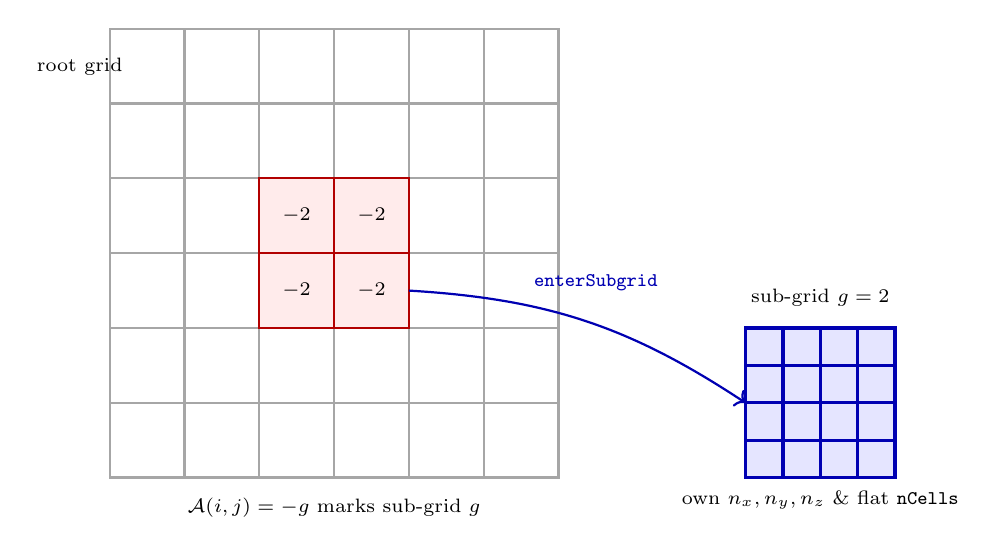
\begin{tikzpicture}[scale=0.95,
   gridcell/.style={draw=gray!70,thick},
   subcell/.style={draw=blue!70!black,very thick,fill=blue!10},
   markercell/.style={draw=red!70!black,thick,fill=red!8}]
  % root grid 6x6
  \foreach \i in {0,...,5}{
    \foreach \j in {0,...,5}{
      \draw[gridcell] (\i,\j) rectangle ++(1,1);
    }
  }
  % red marker cells where active = -2
  \foreach \i in {2,3}{
    \foreach \j in {2,3}{
      \fill[red!8] (\i,\j) rectangle ++(1,1);
      \draw[markercell] (\i,\j) rectangle ++(1,1);
      \node at (\i+0.5,\j+0.5) {\scriptsize $-2$};
    }
  }
  \node at (-0.4,5.5) {\scriptsize root grid};
  \node at (3,-0.4) {\scriptsize $\mathcal{A}(i,j) = -g$ marks sub-grid $g$};
  % sub-grid (4x4 over the 2x2 patch)
  \begin{scope}[xshift=8.5cm]
    \foreach \i in {0,...,3}{
      \foreach \j in {0,...,3}{
        \draw[subcell] (\i*0.5,\j*0.5) rectangle ++(0.5,0.5);
      }
    }
    \node at (1,2.4) {\scriptsize sub-grid $g=2$};
    \node at (1,-0.3) {\scriptsize own $n_x,n_y,n_z$ \&\ flat \texttt{nCells}};
  \end{scope}
  \draw[->,thick,blue!70!black] (4,2.5) to[bend left=15] (8.5,1);
  \node[blue!70!black] at (6.5,2.6) {\scriptsize \texttt{enterSubgrid}};
\end{tikzpicture}
\end{center}

\section{Octree Alternative}

\subsection{Topology}

An octree is a recursive 2$\times$2$\times$2 subdivision of the
computational domain.  The root encompasses the whole simulation volume; any
node may be refined into eight axis-aligned children of equal size.  Nodes
are either \emph{leaves} (carrying physical state) or \emph{internal nodes}
(carrying only topological information).  Each cell sits in a uniquely
defined leaf, and the level of refinement varies from leaf to leaf.

A common variant relaxes the ``one cell per leaf'' rule and instead stores a
small uniform block, typically $4^3$ or $8^3$ cells, inside every leaf.  This
is known as a \emph{block-structured octree} and is the design adopted by
FLASH, Athena++, and ART.  It trades a coarser refinement granularity for
substantially better cache locality and DDA hot-path efficiency.

\subsection{Recommended representation}

A practical implementation combines two views of the same tree:

\begin{enumerate}
\item A \emph{pointer-based} view for traversal,
  \begin{lstlisting}
type :: oct_node
   integer        :: level
   integer(int64) :: morton_key
   real(dp)       :: bbox(6)        ! xmin..zmax
   integer        :: parent
   integer        :: child(8)       ! 0 = leaf
   integer        :: leaf_id        ! index into leaf arrays
   integer        :: owner_rank     ! MPI ownership
end type
type(oct_node), allocatable :: oct_pool(:)
\end{lstlisting}
\item A \emph{Morton-ordered linear} view of the leaves only, used for
  space-filling-curve (SFC) load balancing and for $\mathcal{O}(\log N)$
  point location via binary search on the sorted Morton-key array.
\end{enumerate}

\subsection{Refinement criterion}

Where the patch design relies on the user, the octree picks its leaves from
a refinement function $\mathcal{R}(\text{leaf})$.  Common choices are
\begin{equation}
   \mathcal{R}(\text{leaf}) =
     \alpha \, \frac{|\nabla \log \tau|}{\tau_0}
   + \beta  \, \frac{|\nabla \log n_{\text{H}}|}{n_0}
   + \gamma \, f_{\text{photons}},
\end{equation}
with thresholds for splitting and merging.  At least in a first
implementation it is reasonable to bypass adaptivity entirely and seed the
octree from the user's existing patches: this preserves backwards
compatibility while gaining the unified traversal infrastructure.

\subsection{Ray traversal}

Two well-known algorithms apply.  The \emph{parametric octree traversal} of
Revelles, Ure\~{n}a, and Lastra (2000) sorts the eight children of any
internal node analytically and visits them in the order they are entered by
the ray, without recursion.  Stackless variants, in which one jumps directly
between Morton-key neighbors via bit manipulation, are competitive when the
tree is shallow and well balanced.

In a block-structured implementation the outer loop is octree descent --- in
the hot path, one descent per leaf crossing --- and the inner loop is the
existing 3D-DDA over the leaf's local $4^3$ or $8^3$ cells.  This keeps the
fast inner loop almost identical to the present code.

\subsection{Schematic}

\begin{center}
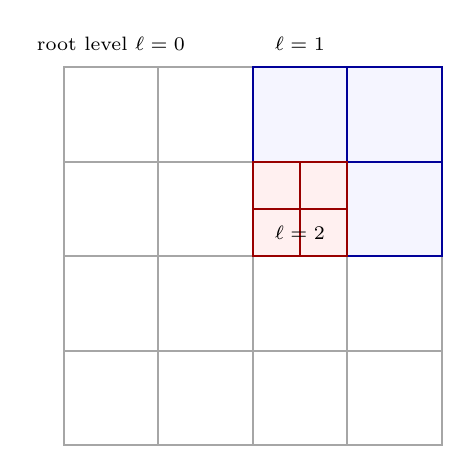
\begin{tikzpicture}[scale=0.6,
  rootcell/.style={draw=gray!70,thick},
  l1cell/.style={draw=blue!60!black,thick,fill=blue!4},
  l2cell/.style={draw=red!60!black,thick,fill=red!6}]
  % a 4x4 root with one quadrant refined to 2x2 and one of those refined again
  \foreach \i in {0,...,3}{
    \foreach \j in {0,...,3}{
      \draw[rootcell] (\i*2,\j*2) rectangle ++(2,2);
    }
  }
  % refine cell (2,2)-(4,4) into 2x2
  \fill[white] (4,4) rectangle (8,8);
  \foreach \i in {0,1}{
    \foreach \j in {0,1}{
      \draw[l1cell] (4+\i*2,4+\j*2) rectangle ++(2,2);
    }
  }
  % refine the lower-left subcell again
  \fill[white] (4,4) rectangle (6,6);
  \foreach \i in {0,1}{
    \foreach \j in {0,1}{
      \draw[l2cell] (4+\i,4+\j) rectangle ++(1,1);
    }
  }
  \node at (1,8.5) {\scriptsize root level $\ell=0$};
  \node at (5,8.5) {\scriptsize $\ell=1$};
  \node at (5,4.5) {\scriptsize $\ell=2$};
\end{tikzpicture}
\end{center}

\section{Side-by-Side Comparison}

\begin{center}
\renewcommand{\arraystretch}{1.15}
\begin{tabular}{p{0.27\textwidth} p{0.32\textwidth} p{0.32\textwidth}}
\toprule
\textbf{Aspect} & \textbf{Patch-based AMR (current)} & \textbf{Octree} \\
\midrule
Refinement granularity
  & whole rectangular patch
  & leaf (1 cell or block of cells) \\
Refinement decision
  & user, static
  & criterion-based, optionally adaptive \\
Tree depth
  & limited by user input (typically 1--3)
  & arbitrary; bounded only by \texttt{maxLevel} \\
Topology storage
  & flat array of grids \texttt{+ motherP}
  & node pool with parent/child pointers \\
Cell $\to$ data lookup
  & $\mathcal{A}(i,j,k)$, $\mathcal{O}(1)$
  & Morton-key binary search, $\mathcal{O}(\log N)$ \\
Cross-grid dispatch
  & sign test on $\mathcal{A}$, helper modules
  & implicit in tree descent \\
Ray traversal
  & 3D-DDA + sub-grid switch events
  & parametric octree, optionally with mini-DDA in blocks \\
MPI partition
  & flat round-robin
  & natural Morton/SFC partition \\
Output
  & grid-by-grid blocks
  & node table + leaf payload \\
Memory pattern
  & grid-wide contiguous (1D \texttt{nCells})
  & leaf contiguous; same shared-window infra reusable \\
Implementation cost
  & $\approx$0 (already in place)
  & 9--11 weeks core path (excluding adaptivity) \\
\bottomrule
\end{tabular}
\end{center}

\section{Why Bother?  When the Equivalence Breaks}

For most existing MOCASSIN runs --- one or two static sub-grids of moderate
size --- the patch design is perfectly adequate, and an octree would only
add overhead.  The case for replacement is concrete in three regimes:
\begin{enumerate}
\item \emph{Multi-scale geometries}.  When the resolution required for the
  ionisation front (or the Str\"omgren boundary, or a dust shadow boundary)
  varies by orders of magnitude across the domain, expressing this as
  rectangular patches forces large unrefined regions to inherit the finest
  resolution of any patch that overlaps them.  Octree refinement is local.
\item \emph{Unknown refinement location}.  If the structure that needs
  resolving is not known a priori --- for example, a moving shock front, or
  the contact discontinuity between a wind and the ambient medium ---
  static patches cannot follow it.  An octree with an adaptivity hook can.
\item \emph{Deep nesting}.  The current dispatch loop is bounded by
  \texttt{nGrids+2}, and the cost of a sub-grid switch is non-negligible.
  At nesting depths beyond three or four, the constant factors begin to
  matter; a unified tree-descent loop scales linearly with depth without
  this overhead.
\end{enumerate}
None of these alone justifies a 2--3 month implementation effort, but in
combination they argue for the move.

\section{Implementation Sketch (cross-reference)}

The detailed eight-phase plan, with file/line targets, regression strategy
and effort estimates, is recorded separately in
\texttt{mocassin-mocassin.2.02.73.2/OCTREE\_PLAN.md}.  Phases at a glance:
\begin{description}
\item[O0] Five upstream design decisions (leaf size, tree representation,
  refinement criterion, dynamic vs.\ static, backwards compatibility).
\item[O1] New \texttt{octree\_mod} with no call sites.
\item[O2] Read-time builder converting existing patch input to an octree;
  consistency assertions only.
\item[O3] Leaf data mirroring the legacy \texttt{nCells} arrays;
  invariant checks each iteration.
\item[O4] Octree ray traversal behind a feature flag; the present DDA path
  remains the truth source.
\item[O5] Optional dynamic refinement criterion.
\item[O6] Morton-SFC MPI redistribution.
\item[O7] Output format extension; backwards compatibility preserved.
\item[O8] Input keywords and final regression matrix.
\end{description}

The principle throughout is that each phase remains bit-identical to the
previous on every existing regression case, and that the octree path is
held to within statistical noise of the patch path on the same nine-case
suite already exercised by Phase~1 and Phase~2.

\section{Conclusion}

The current MOCASSIN refinement design is a flat, statically-defined
collection of rectangular sub-grids stitched together by a sign trick on
the active-cell map.  It is simple, fast, and adequate for most existing
science cases.  An octree replacement would unify the cross-grid dispatch
into a single recursive descent, decouple refinement from user input, and
expose a natural space-filling-curve partition for MPI ---  benefits that
materialise only when the science calls for deep, multi-scale, or
adaptively located refinement.  The transition is well-scoped and
incremental, but it is a real engineering investment; the decision to
undertake it should be driven by a concrete science requirement rather than
by the appeal of the data structure itself.

\end{document}
